\chapter{Materiais e Métodos}
\label{chap:mat}
A criação de uma solução tecnológica vai além de um desenvolvimento e amadurecimento técnico-científico. O olhar sensível a problemática é o primeiro passo para a formação de um conceito. Problemas, desafios, dificuldades sempre existiram e sempre existirão mas a criação de uma solução para estes embates sempre vêm acompanhadas de uma primeira ideia motivadora, subjetiva e totalmente correlacionada às manifestações da natureza humana.

O processo de desenvolvimento de um sistema robótico não é diferente, existe uma motivação da equipe do projeto em cumprir o principal objetivo do conceito arquitetado abordado no capítulo 1. Para garantir que esse objetivo seja alcançado são implementadas metodologias de desenvolvimento de projeto, que ajudam no acompanhamento e definição das atividades como meios para alcançar o fim que é a solução tecnológica.

No sistema de Percepção do robô ELIR a metodologia empregada consiste na divisão do projeto em três principais processos de construção de conhecimento, que são eles : a fase de conceitual e design, a fase de desenvolvimento e a fase de testes. O fluxograma com as fases do projeto está mostrado na Figura \ref{Fig:flux_proj}.

\begin{figure}[h]
	\centering
	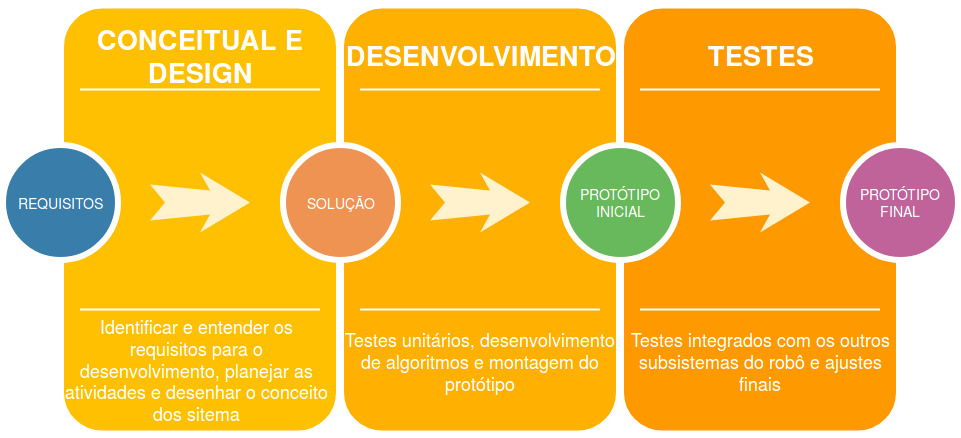
\includegraphics[width=16cm]{Figures/diagrama_proj.jpg}
	\caption{Fluxograma do Projeto}
	\label{Fig:flux_proj}
\end{figure}

O sucesso na execução de um projeto está fortemente relacionada com o seu gerenciamento, organização e planejamento. Por isso, conceitual e design é a fase mais importante do projeto pois ela representa o planejamento e previsão das demais fases. 

Nesta fase, há uma tempestade de ideias a serem organizadas de forma a chegarem em um conceito, um primeiro esboço do que se espera como solução final. Por isso, esta fase é marcada por uma série de reuniões entre a equipe de projeto, o orientador e o cliente a fim de coletar o máximo de informações de requisitos, premissas e necessidades que irão nortear o seu desenvolvimento. Apesar de ser considerada uma fase do projeto ela pode ser quebradas em duas etapas com papéis distintos. O conceitual busca a idealização enquanto o Design busca a avaliação da viabilidade técnica.

A fase de Desenvolvimento é o processo de construção da solução, a qual todas as ideias e planos da fase Conceitual e Design são colocadas em prática. O principal objetivo desta fase é fazer com que as funcionalidades do sistema deixem a área de idealização e se tornem práticas reais e mensuráveis. Por isso, o sucesso desta etapa é relacionado a expertise na fase de Conceitual e Design, nesta fase o planejamento do projeto deve ser fiel às necessidades reais do desenvolvimento.

A última fase do projeto é a fase de Testes. Nesta fase a solução tecnológica é validada por uma série de avaliações estatísticas que quantificam o projeto como todo, seja em desempenho, quanto em função tecnológica.  Esta é a fase de obtenção de resultados e por tanto representa a conclusão do projeto.


\section{Conceitual e Design}
Nesta etapa, a partir das premissas, exclusões, necessidades e definições oriundas das reuniões da equipe de projeto com o cliente e orientador técnico são definidas: A arquitetura geral, especificação funcional,  a arquitetura de software do sistema, os wireframes além dos materiais a serem utilizados.

A arquitetura geral do sistema de Percepção do ELIR é um diagrama de blocos que mostra o fluxo de informações entre os subsistemas da percepção. Ela busca mostrar como as informações são obtidas, como são processadas e como são mostradas. 

A especificação funcional é uma descrição dos processos executados pelo sistema para cumprimento do objetivo geral. Por isso, cada funcionalidade é relacionada a um objetivo específico do projeto mostrado no capítulo 1. Para definição das funcionalidades é necessário descrever o seu objetivo, premissas, descrição, fluxograma de funcionamento e saídas. Esta é a etapa mais relevante da fase Conceitual e Design pois o desenvolvimento é norteado pelas funcionalidades do sistema. 

A arquitetura de Software é um esboço de como as funcionalidades são implementadas no campo de software. Por isso, são definidas as camadas de desenvolvimento e sua relação hierárquica. 

Por último, a definição dos materiais utilizados possui como base dois aspectos principais que são a disponibilidade dos materiais na instituição e a necessidade das funcionalidades do sistema. 


\section{Desenvolvimento}
Na etapa de desenvolvimento são realizadas atividades que tornam o conceito idealizado na fase Conceitual e Design  concreto e factível. Nesta etapa são realizados os testes unitários dos sensores do sistema, o projeto  e fabricação de peças mecânicas para suportar os sensores, são implementados os drivers dos sensores e protocolos de comunicação além da implementação das funcionalidades do sistema e da interface gráfica. 

Os teste unitários dos  sensores do projeto servem para validar o funcionamento e avaliar se suas especificações atendem os requisitos impostos pelo cliente. No teste são coletadas amostras dos dados recebidos de cada sensor e esses dados são avaliados a partir de uma distribuição normal. A distribuição normal assim como qualquer distribuição estatística serve para determinar a probabilidade de ocorrência do fenômeno relacionado a curva. Por isso, é usada no ELIR para avaliação da confiabilidade dos sensores. Ou seja, mostra a probabilidade do sensor se comportar da maneira esperada.

A parte mecânica é projetada para compor todos os sensores que fazem parte do sistema de Percepção, ela representa a integração física do sistema de Percepção no protótipo. Para isso, é necessário estudar as especificações mecânicas de cada sensor do projeto e projetar suportes a serem encaixados na estrutura do robô.

A principal função de um sistema de Percepção é a coleta e tratamento dos dados de seus sensores. Para que estes dados sejam reunidos é necessário que no fim todos os sensores se comuniquem de maneira semelhante, ou seja, utilizando o mesmo protocolo de comunicação. A ferramenta utilizada para a integração destes dados é o framework de robótica. O framework serve para reunir dados de diferentes fontes em um mesmo ambiente, com o mesmo padrão de formatação. Por isso, o desenvolvimento de drivers para cada sensor é extremamente importante pois ele garante a conversão do protocolo de comunicação intrínseco do sensor para o padrão utilizado no framework de robótica.


\section{Testes}
